\ifx\boi\undefined\ifx\problemname\undefined
\providecommand\sampleinputname{}
\providecommand\sampleoutputname{}
\documentclass[nil]{templates/boi}
\ifdefined\babelprovide
  \babelprovide[import=lv,main]{latvian}
\fi
\problemlanguage{.lv}
\fi
\newcommand{\boi}{Baltijas informātikas olimpiāde}
\newcommand{\practicesession}{Izmēģinājuma kārta}
\newcommand{\contestdates}{27.~aprīlis~-- 1.~maijs, 2018}
\newcommand{\dayone}{1.~diena}
\newcommand{\daytwo}{2.~diena}
\newcommand{\licensingtext}{Šis uzdevums ir licencēts zem CC BY-SA~4.0.}
\newcommand{\problem}{Uzdevums}
\newcommand{\inputsection}{Ievaddati}
\newcommand{\outputsection}{Izvaddati}
\newcommand{\interactivity}{Komunikācija}
\newcommand{\grading}{Testēšana}
\newcommand{\scoring}{Vērtēšana}
\newcommand{\constraints}{Ierobežojumi}
\renewcommand{\sampleinputname}{Ievaddatu paraugs}
\renewcommand{\sampleoutputname}{Izvaddatu paraugs}
\newcommand{\sampleexplanation}[1]{#1.~parauga paskaidrojums}
\newcommand{\sampleexplanations}{Paraugu paskaidrojumi}
\newcommand{\timelimit}{Laika ierobežojums}
\newcommand{\memorylimit}{Atmiņas ierobežojums}
\newcommand{\seconds}{s}
\newcommand{\megabytes}{MB}
\newcommand{\group}{Grupa}
\newcommand{\points}{Punkti}
\newcommand{\limitsname}{Ierobežojumi}
\newcommand{\additionalconstraints}{Papildu ierobežojumi}
\newcommand{\testgroups}{%
Jūsu risinājums tiks testēts uz vairākām testu grupām, par katru no tām var iegūt punktus.
Katra testu grupa satur vienu vai vairākus testus.
Lai iegūtu punktus par testu grupu, jums ir pareizi jāatrisina visi testi šajā grupā.
Jūsu beigu vērtējums par uzdevumu būs starp visiem iesūtījumiem lielākais.%
}
\fi
\def\version{jury-1}
\problemname{Maiņstrāva}
Frederiks tagad ir mājās un spēlējas ar paštaisītu rotaļu dzelzceļu, par kuru viņš ir ļoti lepns.
Dzelzceļš sastāv no $N$~segmentiem, kas ir savienoti riņķī un sanumurēti kā $1, 2, \dots, N$ pulksteņa rādītāja virzienā.
Elektrisko strāvu dzelzceļam nodrošina $M$ vadu loki, kas iet līdzi dzelzceļam.
Katram segmentam līdzi iet vismaz viens loks.

Tiesa gan, Frederikam kļūst garlaicīgi skatīties uz riņķojošo vilcienu, tāpēc viņš nolemj pievienot \emph{dzelzceļa pārmiju}
katram segmentam, ko viņš varētu izmantot, lai virzītu vilcienu grāvī un citām aizraujošām lietām.
Pārmijas arī prasa elektrisko strāvu. Un ne jebkādu strāvu — tās prasa tieši \emph{maiņstrāvu}.%
\footnote{Tas ir ļoti loģiski, jo dzelzceļš ir zviedru dzelzceļš~--- un Zviedrijā visas dzelzceļa pārmijas
(``\emph{växlar}'') izmanto maiņstrāvu (``\emph{växelström}'').}

%-- it just moves around in
%circles, and he feels like it could use some more excitement.
%Thus, he comes up with a plan: he will improve things by adding train switches
%to all the segments along the railway. These switches will be hooked up to an
%automatic system that toggles them at random, occasionally causing the train to
%take detours or maybe even go off the rails completely!

%Fredrik has already purchased all the switches he needs for this, but there is one
%remaining problem: the switches also need electricity.

Lai iegūtu maiņstrāvu, Frederiks spriež, ir jābūt strāvai, kas plūst abos
virzienos. Katrs vadu loks dod strāvu tikai vienā virzienā (vai nu pulksteņa rādītāja virzienā,
vai nu otrādi), bet Frederiks var brīvi izlemt, kurā. Secīgi, viņam ir jāizvēlas,
kāds strāvas virziens būs katram lokam, tā, lai katru dzelzceļa segmentu noklāj gan pulksteņa
rādītāja virziena, gan pretējs loks.

Vai jūs varat palīdzēt Frederikam ar šo uzdevumu?

\vspace{2mm}
%\hspace*{2mm}
\begin{center}
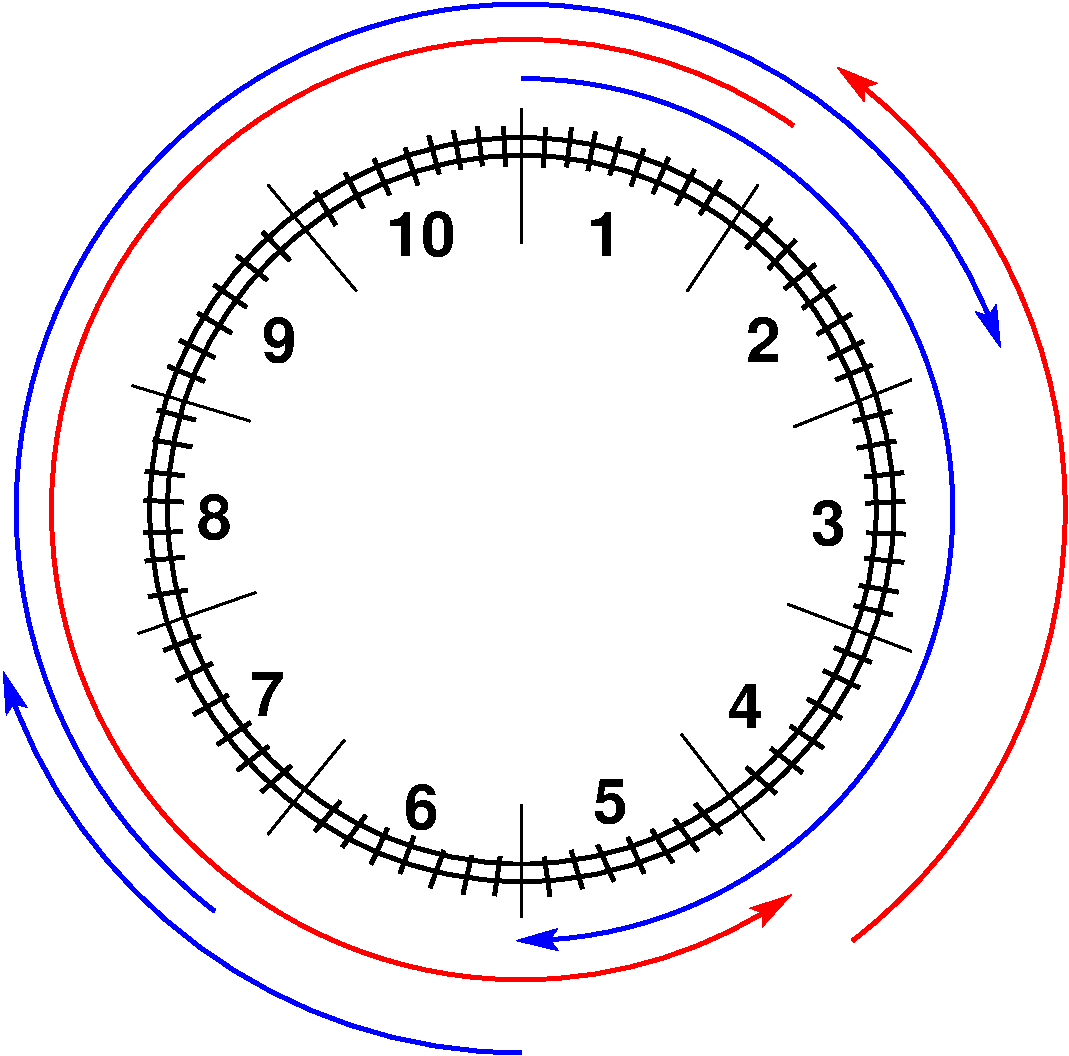
\includegraphics[width=0.5\textwidth]{alternatingfig.pdf}
\end{center}
\vspace{1mm}
\noindent {\em Atrisinājums pirmajam piemēram. Izliektas bultiņas ārpus dzelzceļa apzīmē vadu lokus, kas pievada elektrību. Katras bultiņas virziens ir Frederika izvēlētais elektriskās strāvas virziens (zila un sarkana krāsa apzīmē dažādus virzienus). Ievērojiet, ka visas bultiņas var apvērst pretējā virzienā un iegūt citu pareizu atrisinājumu: \texttt{11010}.}

\section*{\inputsection}
Pirmā rinda satur divus veselus skaitļus~$N$ un~$M$, dzelzceļa segmentu skaitu un loku skaitu, attiecīgi.

Nākamās $M$~rindas katra satur divus skaitļus $1 \le a, b \le N$, kas nozīmē, ka ir vadu loks, kas
noklāj segmentus $a, a+1, \dots, b$. Ja~$b$ ir mazāks par~$a$, tas nozīmē, ka numuri iet pa riņķi,
t.\,i., loks noklāj segmentus $a, \dots, N, 1, \dots, b$. Ievērojiet, ka, ja $a=b$, tad loks noklāj
tikai vienu segmentu.

\section*{\outputsection}
Izvadiet vienu rindu ar $M$~simboliem, katru vai nu \texttt{0}, vai nu \texttt{1}. $i$-jam simbolam rindā
ir jābūt \texttt{0}, ja $i$-tais loks ir orientēts pulksteņa rādītāja virzienā, vai \texttt{1}, ja tas ir orientēts
pretējā virzienā. Ja pastāv vairāki atrisinājumi, izvadiet jebkuru no tiem.

Ja orientēt lokus atbilstoši prasībām nav iespējams, izvadiet ``\texttt{impossible}''.

\section*{\constraints}
\testgroups

\noindent
\begin{tabular}{| l | l | l | l |}
\hline
\textbf{\group} & \textbf{\points} & \textbf{\limitsname} & \textbf{\additionalconstraints} \\ \hline
  1     & 13     & $2 \le N, M \le 15$ & \\ \hline
  2     & 20     & $2 \le N, M \le 100$ & \\ \hline
  3     & 22     & $2 \le N, M \le 1000$ & \\ \hline
  4     & 19     & $2 \le N, M \le 100\,000$ & Nav loku ar $b < a$. \\ \hline
  5     & 26     & $2 \le N, M \le 100\,000$ & \\ \hline
\end{tabular}

